\documentclass[30pt,landscape,magscalefonts]{foils}
\usepackage{floatflt}
%\usepackage{times}
\usepackage{tabularx}
\usepackage[pdftex]{graphicx}
\graphicspath{{./graphics/}}
\usepackage[pdftex]{color}
\usepackage[pdftex]{geometry}
\geometry{headsep=2.0em,hscale=0.80}
\usepackage{hyperref}
\hypersetup{
  pdftitle={SDR 2003 Report on Player},
  pdfauthor={Brian P. Gerkey, USC Robotics Research Lab},
  pdfpagemode={FullScreen},
  pdfborder={0 0 0}
}
%\usepackage{background}

% define some nice colors
\definecolor{myred}{rgb}{0.6,0,0}
\definecolor{myblue}{rgb}{0,0.2,0.4}
% set default background and text colors
%\pagecolor{white}
\color{myblue}

% don't want any paragraph indentation
\setlength{\parindent}{0cm}

% wrapper for foilhead that sets the text color
\newcommand{\foilheadc}[1]{\foilhead{\Large \textcolor{myred}{#1}}\vspace*{-2em}}
% wrapper for itemize that shortens the inter-item separation
\newenvironment{xitemize}{\begin{itemize} \itemsep 1pt}{\end{itemize}}
% wrapper for enumerate that shortens the inter-item separation
\newenvironment{xenumerate}{\begin{enumerate} \itemsep 1pt}{\end{enumerate}}

\def\movieroot{file:///mnt/win/users/gerkey/videos}

\title{\textcolor{myred}
{\large The Player/Stage Project:\\ Making Good Free Software for Robotics
Research}}
\author{\small Brian P. Gerkey\hspace{1.5em} Richard T. Vaughan\hspace{1.5em}
Andrew Howard\vspace*{1em}\\

\includegraphics[height=15mm]{cres-logo.jpg}

\includegraphics[height=15mm]{usclogo.jpg}\hspace*{2em}

\includegraphics[height=15mm]{hrl_logo.jpg} \vspace*{1em}\\
{\tt \small http://playerstage.sourceforge.net}}
\date{}

% headers, etc.
\rightheader{

\includegraphics[height=15mm]{cres-logo.jpg}

\includegraphics[height=15mm]{usclogo.jpg}
}
\leftheader{
\includegraphics[height=15mm]{hrl_logo.jpg}}
\MyLogo{}
\def\totalpages{\pageref{lastpage}}
\rightfooter{\textcolor{myblue}{\quad\textsf{\thepage/\totalpages}}}

\begin{document}

% the title slide
\maketitle

% get the page numbering right
\pagebreak\setcounter{page}{2}

\foilheadc{The problem}
\begin{itemize}
\item Robotics is concerned with the synthesis (and sometimes analysis) of
physical sensor-actuator systems.
\item Interacting with these systems requires a significant amount of
infrastructure:
\begin{itemize}
\item a programmer's interface to robotic devices
\item a simulator
\end{itemize}
\end{itemize}

\foilheadc{The problem (cont'd)}
Good infrastructure for robotics research should be neutral with respect
to:
{\small
\begin{xitemize}
\item language
\item platform
\item architecture
\item hardware
\item location
\end{xitemize}
}
It should also be {\bf Free}.

\foilheadc{Our solution}
The Player/Stage project is a collaborative development effort aimed at
producing high-quality Open Source tools for robotics researchers.

\vspace{1em}
The project primarily maintains two pieces of software:
\begin{itemize}
\item {\bf Player}: A networked robot device server.
\item {\bf Stage}: A multiple robot simulator.
\end{itemize}

\foilheadc{Usage}
\begin{center}
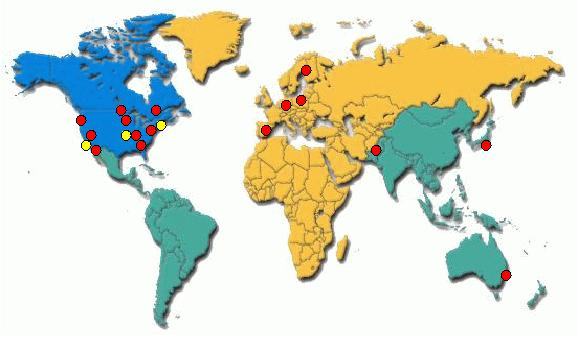
\includegraphics[height=130mm]{usage-map.jpg}
\end{center}

\foilheadc{Usage (cont'd)}
\begin{center}
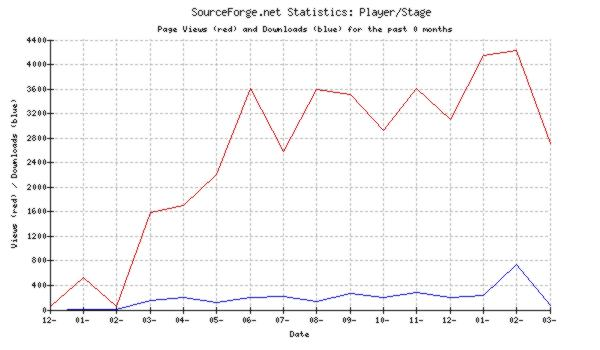
\includegraphics[height=130mm]{stats_graph_blur.jpg}
\end{center}

\foilheadc{Supported hardware / software}
{\small
\begin{itemize}
\item {\bf Robots}: ActivMedia, RWI, K-Team
\item {\bf Laser}: SICK LMS 200
\item {\bf PTZ}: Sony EVID30
\item {\bf IMUs}: Microstrain 3DM-G IMU, ISense InertiaCube2
\item {\bf Wifi}: linuxwifi, iwspy, aodv
\item {\bf Vision}: ACTS, CMVision
\item {\bf Speech}: Festival
\end{itemize}
}

\foilheadc{Player architecture}
\begin{center}
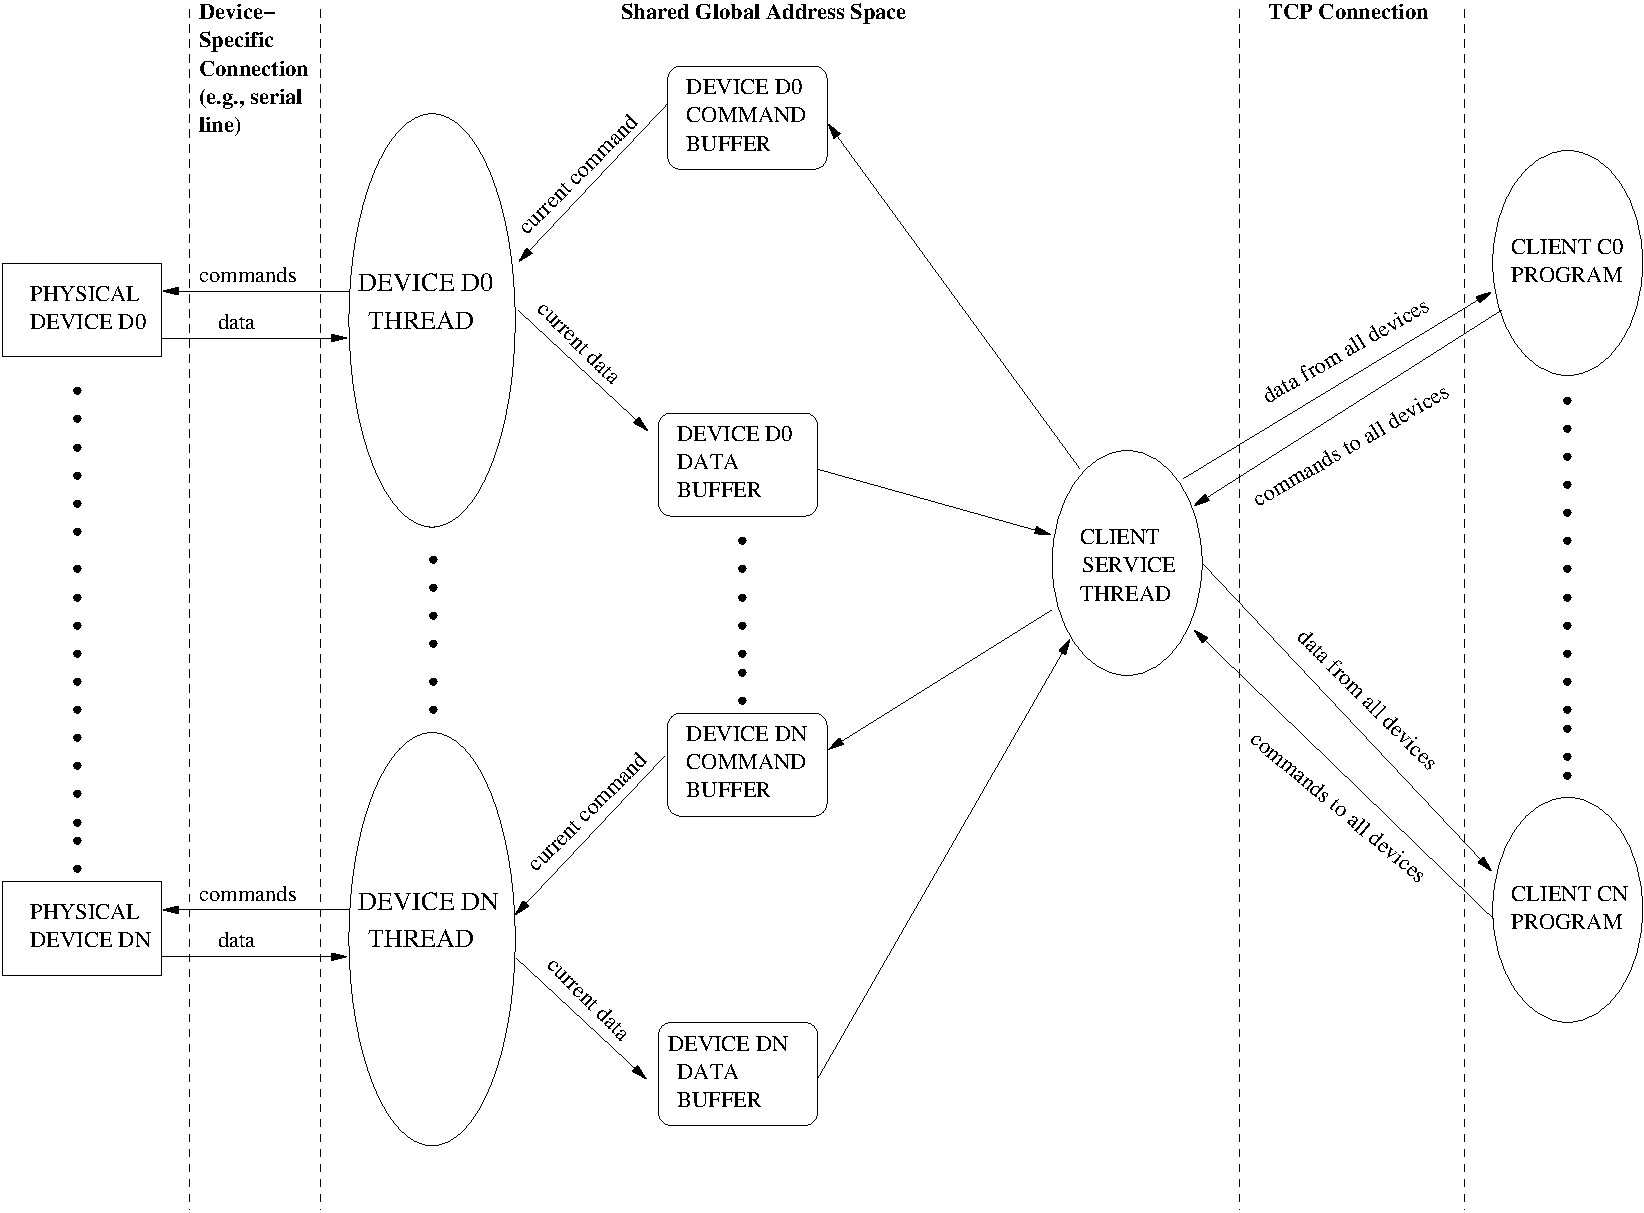
\includegraphics[height=130mm]{buffers.pdf}
\end{center}

\foilheadc{Player design}
Player is built on 3 key abstractions, borrowed from operating systems
design:

\begin{tabular}{cc}
\parbox{.6\textwidth}{
\begin{itemize}
\item read/write/ioctl model
\item \fbox{interface/driver model}
\item client/server model
\end{itemize}}
&
\parbox{.3\textwidth}{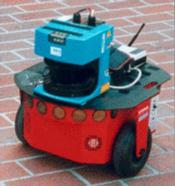
\includegraphics[width=.3\textwidth]{pioneer-2-small.jpg}}
\end{tabular}

\foilheadc{Interfaces vs.\ drivers}
\begin{xitemize}
\item A device {\em interface}, such as {\bf sonar}, is a generic
specification of the format for data, command, and configuration
interactions.
\item A device {\em driver}, such as {\bf pioneer-sonar} or {\bf
rwi-sonar}, specifies how the low-level device control will be carried
out.
\item Multiple drivers can present the same interface.
\item The {\bf same} controller can be used with {\bf different} devices.
\end{xitemize}

\foilheadc{Sophisticated drivers}
{\small
\begin{itemize}
\item Drivers can do much more than provide transparent access to a device.
\item Arbitrary computation can be embedded in a driver.
\item Well-understood algorithms can be encapsulated in Player and
offered as standard services.
\item Examples: acoustic filtering, probabilistic localization.
\item Player becomes a community code repository.
\end{itemize}
}

\foilheadc{Sophisticated drivers (cont'd)}
The {\bf laser-visual fiducial-finder}:

\begin{tabular}{cc}
\parbox{.7\textwidth}{
\begin{itemize}
\item Uses laser range-finder, PTZ camera and color segmenter to locate and 
identify fiducials.
\item Performs sensor fusion on range and image data.
\item Includes closed-loop control of PTZ camera.
\end{itemize}}
&
\parbox{.3\textwidth}{\href{\movieroot/lvb.avi}{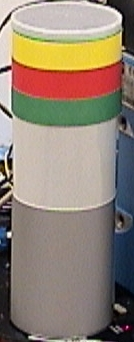
\includegraphics[width=.21\textwidth]{laservisualbeacon2.jpg}}}
\end{tabular}

\foilheadc{Shifting the computation}
\begin{xitemize}
\item When an algorithm is implemented as a driver, the associated
computational load is moved to the server.
\item The {\bf passthrough} driver acts as a proxy within one server
for a device in another server.
\item Allows computational load to be shifted arbitrarily, within a
network or across the Internet.
\item Also allows one server to aggregate and distribute data and
commands for multiple robots.
\end{xitemize}


\foilheadc{Stage: a multi-robot simulator}
Provides a population of virtual Player devices.
\begin{xitemize}
\item All devices controlled through Player.
\item Robots move in two-dimensional bitmapped world.
\item Models designed to scale to large populations.
{\small
\begin{itemize}
\item Computation scales linearly with P.
\item User specifies world resolution.
\item 200 robots w/ sonar, odometry, etc.
\item 20 robots w/ color blobs, laser scanner.
\end{itemize}
}
\end{xitemize}

\foilheadc{Stage (cont'd)}
\begin{xitemize}
\item Models present the {\bf Player Abstract Device Interface (PADI)}.
\item In many cases, Player clients produce similar behavior in Stage and with
the real devices.
\item Controllers have been shown to transition from simulation to hardware
(and back) with almost no changes.
\item Results obtained with Stage are gaining respect in the research
community.
\end{xitemize}

\foilheadc{Modeled hardware}
\begin{center}
\href{\movieroot/stage-everything.mpg}{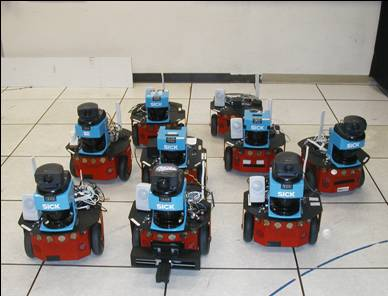
\includegraphics[height=130mm]{uscpioneers.jpg}}
\end{center}


\foilheadc{World description file}
{\tiny
\begin{verbatim}
bitmap (
  file "hospital.pnm.gz"
  resolution 0.03
)

define pioneer2dx position (
  size [.440 .330]
  offset [-0.04 0.0]
  p2dx_sonar()
  broadcast ()
  laser()
  gripper()
)

pioneer2dx (robot 1 color "blue"  pose [1.0 1.0  -90])
pioneer2dx (robot 2 color "green" pose [1.5 1.0    90])
pioneer2dx (robot 3 color "red"   pose [1.9 0.8 -110])

puck( color "red" pose [1.4 0.5 0.0] )
\end{verbatim}
}

\foilheadc{Disruptive technology?}
{\small
\begin{xitemize}
\item Standard set of devices
\item Standard device abstractions
\item Standard transport (client$\leftrightarrow$device comms)
\item Standard sensor processing devices
\item Standard environments
\item Standard tasks
\item Standard metrics
\end{xitemize}
}

$\Rightarrow$ compare your control techniques with others

\foilheadc{Player Abstract Device Interface (PADI)}
\begin{itemize}
\item Some Player interfaces are now supported by multiple hardware devices and
      Stage models.
\item Portable, reusable code runs on multiple devices.
\item Emerging as a virtual machine for mobile robotics that is open, free, 
      and supported by multiple vendors' platforms.
\end{itemize}

\foilheadc{PADI (cont'd)}
\begin{itemize}
\item Challenge: define a set of widely useful interface descriptions that:
\begin{itemize}
\item group functionally similar devices
\item have complete, consistent semantics
\end{itemize}
\item Robotics Engineering Task Force (RETF): an effort underway to develop
standard robotics protocols / APIs (like we have for networks).
\end{itemize}

\foilheadc{\small {\tt hospital.world}, Fort Sam Houston, TX}
\begin{center}
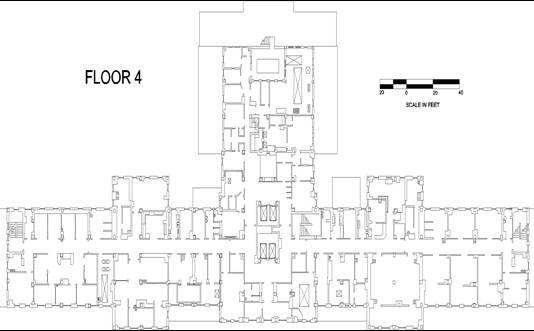
\includegraphics[height=130mm]{hospital.jpg}
\end{center}

\foilheadc{Online multi-player\\ robot simulation}
Provide persistent online server:
\begin{xitemize}
\item Connect to a pool of pre-created devices, or
      create devices from the available models.
\item Users can only perceive the world through Player.
\item Optional world-per-experiment or shared-world.
\item Stage logs behavior and measures performance.
\end{xitemize}

\foilheadc{Online multi-player robot simulation (cont'd)}
Candidate task challenges:
{\small
\begin{xitemize}
\item Multi-robot tracking and surveillance
\item Mapping
\item Target finding speed challenge
\item Autonomy challenge
\begin{xitemize}
\item Create an energy economy.
\item Robots must act to maintain their existence and perform a useful
task.
\end{xitemize}
\end{xitemize}
}

\foilheadc{Player: future work}
\begin{xitemize}
\item Simultaneous localization and mapping.
\item Device name-server / discovery.
\item More closed-loop control:
\begin{xitemize}
\item Impedance controller
\item Target-tracking (visual servoing)
\item Waypoint-following
\item Wall-following
\item Formation-maintenance
\end{xitemize}
\end{xitemize}

\foilheadc{Stage: future work}
{\small
\begin{xitemize}
\item Stage server handles clients over a socket.
\item Dynamically add, remove, configure models.
\begin{xitemize}
\item Tweak all model properties online.
\end{xitemize}
\item Models present pure PADI.
\begin{xitemize}
\item Plus optional extensions to provide device-specific ioctls.
\end{xitemize}
\item More powerful, general base model, e.g.:
\begin{xitemize}
\item Model bodies composed from arbitrary rectangles, lines, arcs, ellipses,
bitmaps with full collision detection.
\item Mass and acceleration support.
\end{xitemize}
\end{xitemize}
}

\foilheadc{Summary}
\begin{xitemize}
\item All Player/Stage software is Open Source, released under the GNU GPL.
\item P/S run on many OSs (e.g., Linux, Solaris, OS~X, FreeBSD)
\item Player runs on many embedded systems 
(e.g., ipEngine, nanoEngine, XScale, iPAQ).
\item Player supports (and Stage models) many common research robots and 
peripherals.
\end{xitemize}

\foilheadc{Acknowledgments}
{\tiny
{\bf Developers}:
Maxim Batalin, Josh Bers, Brendan Burns, Jason Douglas, Jakob Fredslund,
Brian Gerkey, Andrew Howard, Kim Jinsuck, Boyoon Jung, Alex Makarenko, Andy
Martignoni III, Nik Melchior, Dave Naffin, Esben \O{}sterg\aa{}rd, Gabe Sibley,
Kasper St\o{}y, John Sweeney, Doug Vail, Richard Vaughan\\
{\bf Support}:
Maja Matari\'{c} \& Gaurav Sukhatme @ USC, Dave Payton @ HRL\\
{\bf Project management}: SourceForge.net
}
\begin{center}
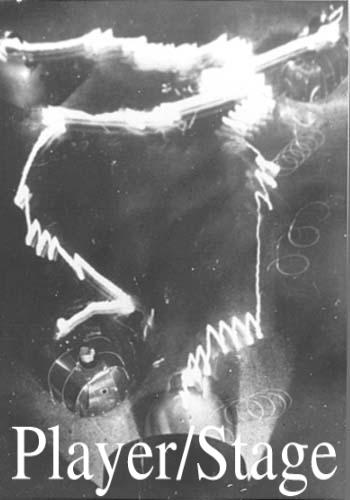
\includegraphics[height=40mm]{ps_logo.jpg}\\
\fbox{\small \tt http://playerstage.sourceforge.net}
\end{center}

\foilheadc{Another movie}
\label{lastpage}
\vfill
\begin{center}
\href{\movieroot/stage-table.mpg}{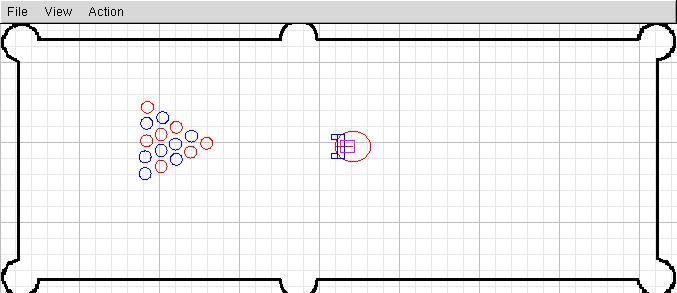
\includegraphics[width=\textwidth]{stage-table.jpg}}
\end{center}
\vfill

\end{document}
